\documentclass[12pt]{article}
% font setup, use Lualatex to compile!
\usepackage{fontspec}
% page margin
\usepackage[inner=2.54cm,outer=2.54cm]{geometry}
% change caption as I WANT
\usepackage{caption}
% initialize image referencing
\usepackage{graphicx}
\graphicspath{ {images/} }
\usepackage{caption}
\usepackage{subcaption}
% allows landscape figure
\usepackage{rotating}
% footers and headers
\usepackage{fancyhdr}
\pagestyle{fancy}
\fancyhf{}
\chead{\textit{MY TITLE in the Head}}
\rfoot{\thepage}
\lfoot{\textit{Date - Month - Year}}
\renewcommand{\headrulewidth}{0pt}
\renewcommand{\footrulewidth}{0pt}

% Matlab code block
\usepackage[T1]{fontenc}
\usepackage{bigfoot} % to allow verbatim in footnote
\usepackage[numbered,framed]{matlab-prettifier}
\usepackage{filecontents}
\let\ph\mlplaceholder % shorter macro
\lstMakeShortInline"
\lstset{
  style              = Matlab-editor,
  basicstyle         = \mlttfamily,
  escapechar         = ",
  mlshowsectionrules = true,
}

% initialize clickable references
\usepackage[unicode]{hyperref}
\hypersetup{
    colorlinks,
    citecolor=black,
    filecolor=black,
    linkcolor=black,
    urlcolor=black
}
% reference styles
\usepackage[style=ieee, natbib=true]{biblatex}
\addbibresource{refs.bib}
% appendices
\usepackage{appendix}
% initialize math tools
\usepackage{amsmath}
\usepackage{amssymb}
\usepackage{empheq}
\usepackage{bm}
% allow newline in cells of table
\usepackage{makecell}
% define sign convention
\makeatletter
% no indentation
\setlength\parindent{0pt}

\newcommand*\curveplus{%
  \mathbin{\rotatebox[origin=c]{90}{$\m@th\curvearrowleft$}+}}

\newcommand*\rightplus{%
  \mathpalette\@rightplus\relax}
\newcommand*\@rightplus[1]{%
  \mathbin{\vcenter{\hbox{$\m@th\overset{#1+}{\to}$}}}}

\newcommand*\upplus{%
  \mathbin{+\mathord\uparrow}}

\makeatother
% add indentation
\usepackage[parfill]{parskip}
% abstract lines
\usepackage{geometry}
\usepackage{lipsum}
\renewenvironment{abstract}
 {\quotation\small\noindent\rule{\linewidth}{.5pt}\par\smallskip
  {\centering\bfseries\abstractname\par}\medskip}
 {\par\noindent\rule{\linewidth}{.5pt}\endquotation}


\begin{document}
    \title{MY TITLE}
    \author{Name, zID\\\small \textit{PSS Group: Friday / 1200-1400 / EE G03}}
    \date{}
    \maketitle
    \begin{abstract}
       blah blah blah
    \end{abstract}

\section{Introduction}
\label{sec:Introduction}
    The purpose of this lab is to explore the fundamentals of ...

        \begin{figure}[h]
            \centering
            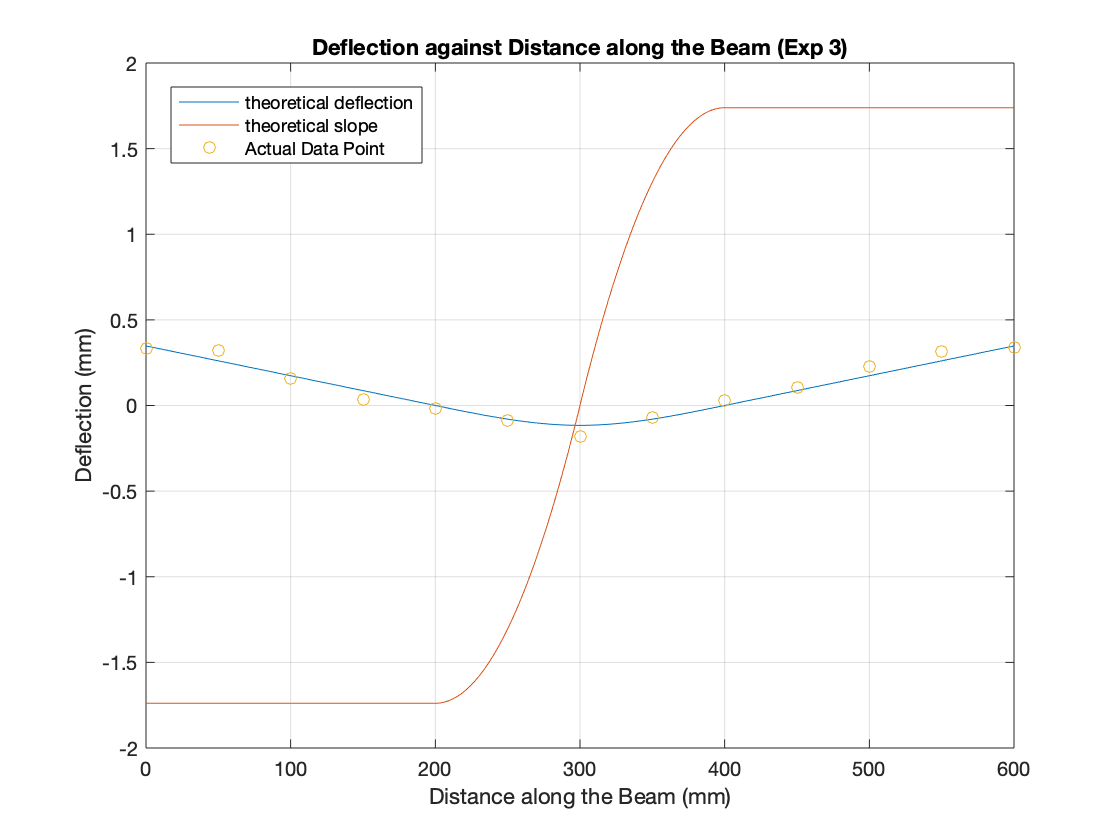
\includegraphics[width=0.9\textwidth]{delta_against_distance.png}
            \caption{\label{fig:delta_against_distance}Deflection against Distance along the beam for experiment 3.}
        \end{figure}
       
        \begin{table}[h]
            \centering
            \caption{\label{tab:Youngs_modulus_comparison} Comparison of experimentally obtained Young's moduli with standard values.}
            \begin{tabular}{|c|c|c|}\hline
                 & Young's Modulus & $|\%\epsilon|$ \\\hline
              Experiment 1 & 117.087 GPa & 3.160 \\\hline
              Experiment 4 & 114.691 GPa & 1.049 \\\hline
              Standard E \cite{common_values} & 113.5 GPa & 0 \\\hline
            \end{tabular}
        \end{table}

% \printbibliography[heading=bibintoc, title={References}]
\clearpage
\appendix
\section*{Appendix}
\section{Calculation}
\label{sec:A-calculation}
    The second moment of inertia of the specimen plate is found by
    \begin{align}
        \label{eq:second_moment_inertia}
        \begin{split}
            I &= \frac{b h^3}{12}\\
            &= \frac{19\cdot3.15^3}{12}\cdot10^{-12}\\
            &=4.94885\cdot10^{-11}\,\,\text{m}^4\\
        \end{split}
    \end{align}

\end{document}
